\section{Diskussion og lyttetest}

\subsection{Lyttetest}
Da god lyd, eller bedre lyd er en objektiv holdning, har gruppen valgt at lave en lyttetest. I denne lyttetest, vil resultatet give os en indikation, om Jazz konfig, og Rock konfig, har den ønskede effekt. Testen er lavet på 13 personer. Grundet tidspres, er testen lavet som en udvidet "kan-du-høreforskel" test, hvor testpersonaerne blot skal give indikation om hvilken afspilning der er bedst. Dette betyder også at normalfordeling og spredning ikke kan laves på testen. Testen er derfor en test af trends, altså af hvad der lyder bedst. Herunder vil der beskrives en gennemgang af testen, og på figur \ref{fig:Lyttetest} kan ses den test, som blev udleveret til hver af test deltagerne.  
 
\subsubsection{selve testen}
Testen er udført som en AB test, hvor der er tilføjet et C (ABC test), dette betyder at testpersonerne hører 3 konfigationer af hver musikklip, hvorefter testpersonen skal vælge hvilken af de 3 konfigarationer som er bedst. Deltagerne kommer skiftevis ind i lytterummet, en af gangen, og bliver presenteret for de 3 genrer. For at undgå bias i testen, er der valgt en version A og B, som har hver deres rækkefølge. lydniveauet for alle deltagerne er ens, og der er ikke taget højde for hverken alder eller køn.    

\subsubsection{Programmateriale}
De tre sange er som følge: \\
Jazz: Max Roach \& Abbey Lincoln - Lonesome Lover \\
Rock: ACDC - Thunderstruck \\
Pop: Taylor Swift - 22 \\
Disse sange er valgt ud fra, at de er forholdsvis kendte, og rammer deres genrer. Hver af sangene er klippet, så det varer 15 sekunder et sted i sangen omkring omkvædet. 

\subsubsection{Resultat}
På figur \ref{fig:lytteresultat} ses resultatet af testen. Her ses flere forskellige tendenser:  \\Jazz musikken har ingen klare tendenser, dette betyder at vores jazz konfiguration ikke har haft den ønskede virkning, som var at forbedre kvaliteten af jazz musik. \\Rock musikken har en klar tendens, nemlig at 8 ud af 13 testpersoner (61\%) foretrækker rock konfigurationen ift de to andre. Herved ses at rock konfigurationen har den positive trend som var målet for udviklingsholdet. \\
Pop musikken var taget med for at teste om standart filteret var bedst, når ingen af de to musikgenrer, som var lavet forbedringer på, optrådte. Her ses igen en tendens, som indikerer at vores standart filter viser den største trend indenfor pop. 
 
\begin{figure}[H] 
	\center
	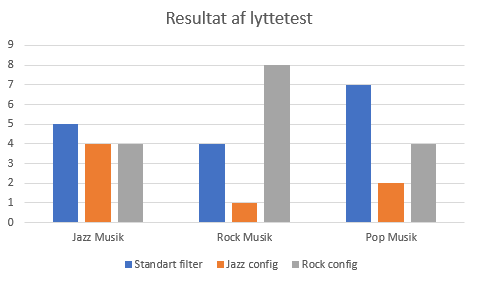
\includegraphics[width=0.8\linewidth]{figur/lytteresultat}\quad
	\caption{Resultat af lyttetesten}
	\label{fig:lytteresultat}
\end{figure}
Samlet set er prodjektgruppen tilfreds med resultatet, da rock configurationen er den mest populære blandt rock nummeret. Derudover er standart filter populær blandt alle genrer, hvilket også er tilfredsstilende ift. projektgruppen, da standart filteret skulle passe til alt musik. På den negative side, vurderes jazz configurationen ikke til at leve op til de forventninger projektgruppen havde til configurationen.  


\subsection{Diskussion}
Igennem processen af produktet, mødte gruppen flere udfordringer. Da projektet omhandler højtalere som gruppen ingen data havde på, kom der problemstillinger ift målinger. Den første udfordring kom herved, at ved måling af frekvensresponsen, blev afstanden mellem højtaler og mikrofon lavet ud fra afstandsmåling med tomstok. For at sikre at hver måling var ens, skulle gruppen have lavet en opstilling som altid stod ens. Hertil blev nogle af målingerne lidt forskellige, da opstilligen ikke var 100\% ens. \\ \\
Gennem optimeringsfasen forsøgte gruppen af lave frekvensresponsen så flad som muligt. Efter målingen af diskanten og basenheden, valgte gruppen at lave et crossover filter ved 4 kHz og hertil et optimeret filter. Ifølge målingerne burde dette give et stort set fladt frekvensrespons. Efter højtalerne blev placeret i kabinettet, blev frekvensresponsen dog en smule ændret, som det ses på figur \ref{fig:Optimering-forskel}. Dette er sandsynligvis et resultat af kabinnettets resonansfrekvens, og stående bølger inde i kabinettet, og et resultat af at bruge et kabinet som ikke er designet til præcis disse enheder. \\ \\
Ideen bag de to konfigurationer var, at forstærke og dæmpe bestemte frekvenser ift hvilke instrumenter som indgår i musikgenren. Dette gav dog den problemstilling, at ved at ændre forstækningsforholdene på baggrund af et bestemt instrument, muligvis forstærkede negative effekter for andre instrumenter. Dette er også grunden til at man normalt i et lydstudie retter hvert instrument til, for at få det bedste fra hvert instrument. Ud fra lyttetesten, ses at de negative effekter ved jazz configurationen, kan være årsag til den ikke er at foretrække. Modsat ses ved rock configurationen, at de tilsigtede effekter har en virkning på lydoplevelsen. \\ \\
Lyttetesten er lavet for at verificere nogle af de pointer og tiltag som de to configurationer er lavet ud fra. Hvis gruppen havde haft mere tid, og flere forsøgspersoner, ville fokusset være på at lave en test ud fra nogle subjective parametre. Her kunne parametre som fullness og crispness være nogle af de parametre som kunne testes. Hertil ville der også kunne laves en skala, så man kunne lave normalfordeling og spredning på resultaterne.\\ En anden vinkel, gruppen kunne have sat i fokus, var at repetere den samme sekvens af de 3 lydklip, for at se om besvarelser var tilfældige eller deterministiske<. Herudover kunne man også tilføje flere musik numre, af samme genrer, for at verificere at resultatet er gængs over forskellige numre. 

      
